\documentclass[aspectratio=169]{beamer}

\usepackage{beamertheme-custom}
\usepackage{symbols-custom}
\usepackage{ 
    enumitem,
    booktabs,
    tikz,
    tikz-qtree,
    xcolor,
    graphicx}
\graphicspath{{figures/}}
\usetikzlibrary{trees}
\usetikzlibrary{tikzmark}

\title{Cultural Consensus Theory}
\author{Joachim Vandekerckhove}
\date{Spring 2025}

\tikzset{% set up for transitions using tikz with beamer overlays
  invisible/.style={color=black!75!white},
  color on/.style={alt=#1{}{invisible}},
  alt/.code args={<#1>#2#3}{%
    \alt<#1>{\pgfkeysalso{#2}}{\pgfkeysalso{#3}} % \pgfkeysalso doesn't change the path
  },
}

\setlist[enumerate]{label=\bf\alph*)}
\setbeamercolor{item}{fg=black}

\usefonttheme[onlymath]{serif}
\beamerdefaultoverlayspecification{<+->}

% Disable metropolis minimal itemize override
\setbeamertemplate{itemize items}[default]

\setbeamertemplate{itemize item}{\textbullet} % or \ding{43}, etc.
\setbeamertemplate{itemize subitem}{--}
\setbeamertemplate{itemize subsubitem}{$\ast$}
\setlist[itemize]{label=$\bullet$}

\begin{document}

\maketitle


\begin{frame}
    \frametitle{What Do Groups ``Know''?}
    \begin{itemize}
        \item How can we identify and measure shared knowledge or beliefs within a community?
        \item How can we distinguish shared knowledge from individual variation, error, or differing opinions?
        \item Traditional methods often rely on subjective assessments.
        \item Need: A formal, \textit{quantitative} approach to shared cognition.
    \end{itemize}
\end{frame}


\begin{frame}
    \frametitle{Cultural Consensus Theory (CCT)}
    \begin{itemize}
        \item A statistical model to infer shared cultural knowledge or shared beliefs from individual responses.
        \item Developed by anthropologists and cognitive scientists in the early 1980s (notably, Romney, Weller, and Batchelder)
        \item \textit{Core assumptions of original CCT:} 
        \begin{itemize}
            \item There exists a ``common truth''
            \item Informants respond independently of one another
            \item Items are homogeneous (equally difficult to a respondent with fixed competence)
        \end{itemize}
        \item In other words, individuals will tend to agree more with each other and with the ``truth'' if they understand the domain.
    \end{itemize}
\end{frame}


\begin{frame}
    \frametitle{Derivations from the model (Romney et al., 1986)}
    \begin{figure}
        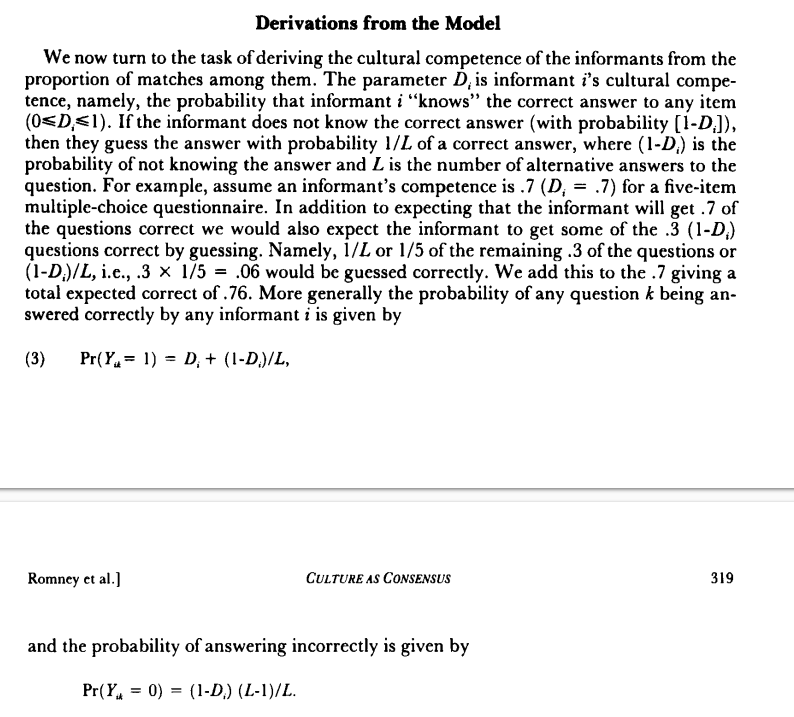
\includegraphics[width=0.8\textwidth,trim=0 340 0 0,clip]{figures/romney.png}
        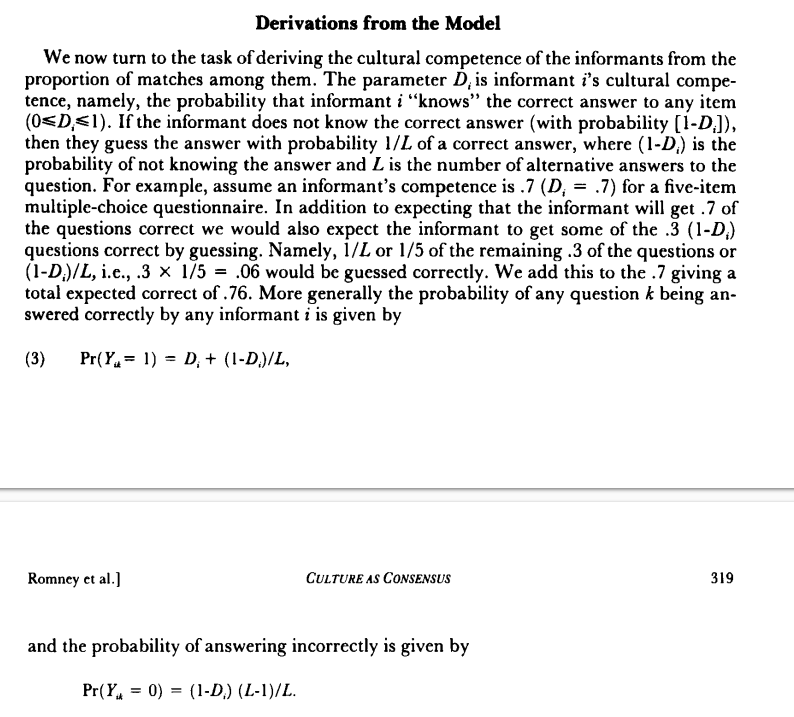
\includegraphics[width=0.8\textwidth,trim=0 0 0 620,clip]{figures/romney.png}
    \end{figure}
\end{frame}


\begin{frame}
    \frametitle{Derivations from the model (Romney et al., 1986)}
    \begin{figure}
        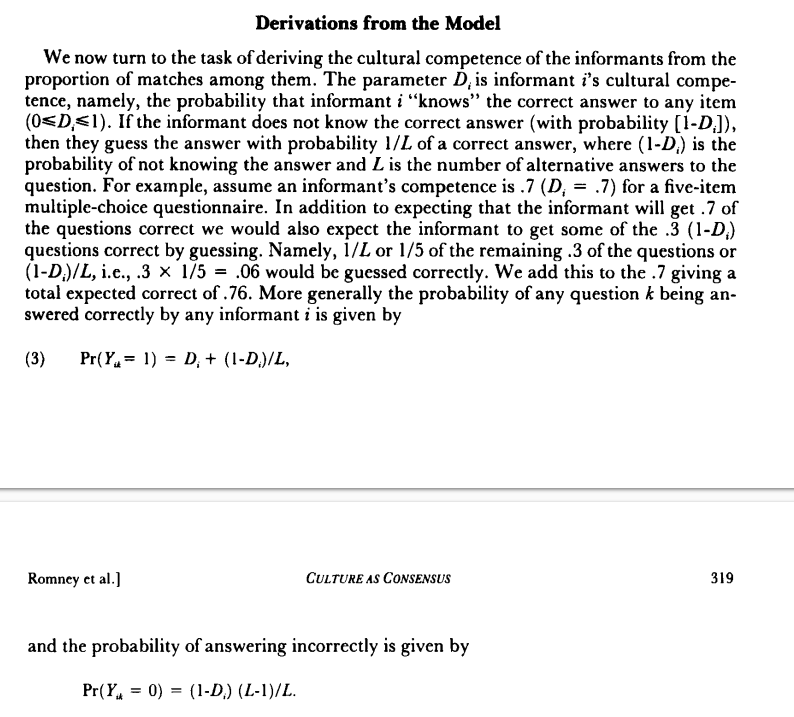
\includegraphics[width=0.8\textwidth,trim=0 340 0 330,clip]{figures/romney.png}
        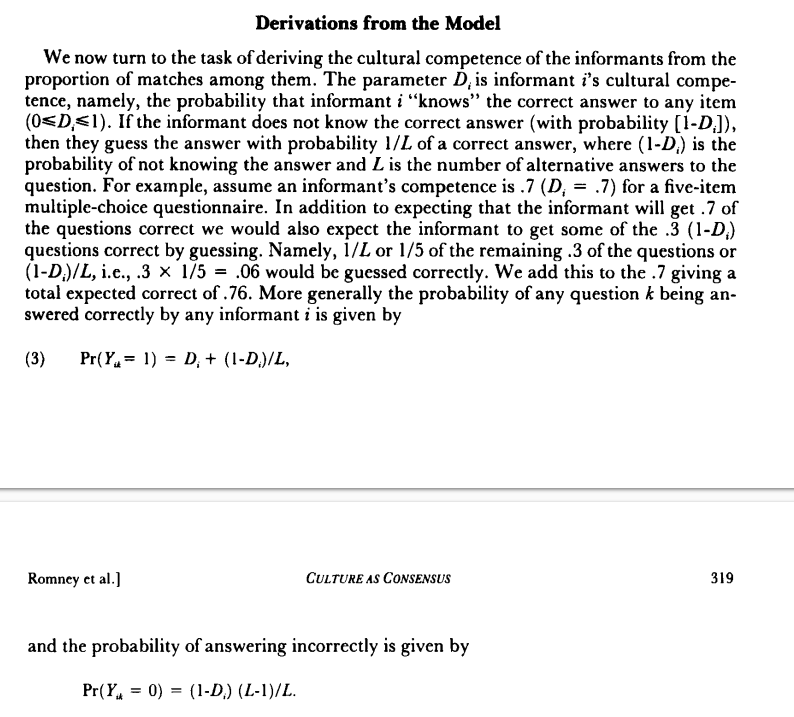
\includegraphics[width=0.8\textwidth,trim=0   0 0 620,clip]{figures/romney.png}
    \end{figure}
    
    These equations might look familiar.\pause

    \begin{center}
      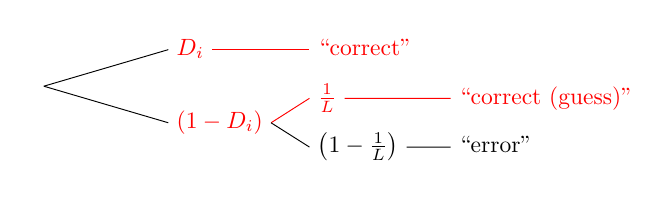
\begin{tikzpicture}[scale=0.85]
\tikzset{grow'=right}
\tikzset{execute at begin node=\strut}
\tikzset{every tree node/.style={anchor=base west}}
\tikzset{level 1/.style={level distance=60pt}}
\tikzset{level 2/.style={level distance=60pt}}
\tikzset{level 3+/.style={level distance=60pt}}
\Tree [.{} [.\node[color=red,color on=<3->]{$D_i$};\edge[draw=red,color on=<3->]; \node[color=red,color on=<3->]{``correct''}; ]
              		[.\node[color=red,color on=<4->]{$\left(1-D_i\right)$}; \edge[draw=red,color on=<4->];	[.\node[color=red,color on=<4->]{$\frac{1}{L}$}; \edge[draw=red,color on=<4->]; \node[color=red,color on=<4->]{``correct (guess)''};  ]
						[.$\left(1-\frac{1}{L}\right)$ ``error'' ]
 ] ] 
\end{tikzpicture}
    \end{center}
    
\only<5>{Of course we don't know which answers are ``correct''!}
\end{frame}

\begin{frame}
    \frametitle{Derivations from the model (Romney et al., 1986)}
    \vspace{1ex}
    
    Let's instead think about the data $Y_{ij}$ of participant $i$ on item $j$, and let's focus on True/False questionnaires (so $L=2$, and $T_j=1$ if $j$ is really true).\pause
    
    If participant $i$ ``endorses'' item $j$, then $Y_{ij} = 1$.  How many ways can they endorse it?\pause
    
    \begin{center}
      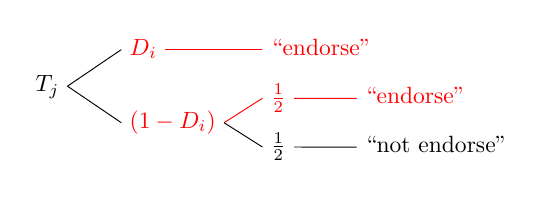
\begin{tikzpicture}[scale=0.85]
\tikzset{grow'=right}
\tikzset{execute at begin node=\strut}
\tikzset{every tree node/.style={anchor=base west}}
\tikzset{level 1/.style={level distance=40pt}}
\tikzset{level 2/.style={level distance=60pt}}
\tikzset{level 3+/.style={level distance=40pt}}
\Tree [.{$T_j$} [.\node[color=red]{$D_i$};\edge[draw=red]; \node[color=red]{``endorse''}; ]
              		[.\node[color=red]{$\left(1-D_i\right)$}; \edge[draw=red];	[.\node[color=red]{$\frac{1}{2}$}; \edge[draw=red]; \node[color=red]{``endorse''};  ]
						[.$\frac{1}{2}$ {``not endorse''} ]
 ] ] 
\end{tikzpicture}
      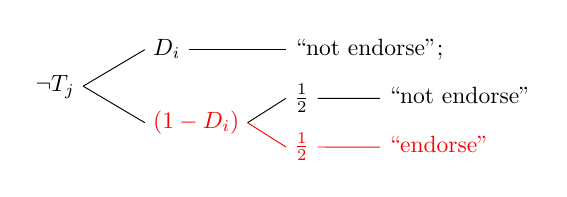
\begin{tikzpicture}[scale=0.85]
\tikzset{grow'=right}
\tikzset{execute at begin node=\strut}
\tikzset{every tree node/.style={anchor=base west}}
\tikzset{level 1/.style={level distance=50pt}}
\tikzset{level 2/.style={level distance=60pt}}
\tikzset{level 3+/.style={level distance=40pt}}
\Tree [.{$\lnot T_j$} [.\node{$D_i$};\edge; {``not endorse''}; ]
              		   [.\node[color=red]{$\left(1-D_i\right)$}; \edge;	[.\node{$\frac{1}{2}$}; \edge; \node{``not endorse''};  ]
					   \edge[draw=red];	[.\node[color=red]{$\frac{1}{2}$}; \edge[draw=red]; \node[color=red]{``endorse''};  ]
 ] ] 
\end{tikzpicture}
    \end{center}
\vspace{-2ex}\pause
\begin{eqnarray*}
P\left(Y_{ij} = 1\right) &=& T_j\left(D_i + \left(1-D_i\right)\frac{1}{2}\right) + \left(1-T_j\right)\left(1-D_i\right)\frac{1}{2}\\
                         &=& T_jD_i + \left(1-D_i\right)\frac{1}{2}
\end{eqnarray*}

\end{frame}


\begin{frame}
    \frametitle{Guessing and acquiescence}
    
$$P\left(Y_{ij} = 1\right) = T_jD_i + \left(1-D_i\right)\frac{1}{2}$$

We made the simplifying assumption just now that $L=2$.  Using the diagrams on the previous slide, convince yourself that this assumption was \emph{without loss of generality} (WLOG) -- that is, the same logic is true if $L > 2$.\pause

Specifically:
$$P\left(Y_{ij} = 1\right) = T_jD_i + \left(1-D_i\right)\frac{1}{L}$$\pause

We might even say that respondents have an individual bias $g_i$ towards endorsing anything (``acquiescence bias''):
$$P\left(Y_{ij} = 1\right) = T_jD_i + \left(1-D_i\right)g_i$$

\end{frame}


\begin{frame}
    \frametitle{Simplifying a little}
    
    Let's take out the guessing for now
    \begin{center}
      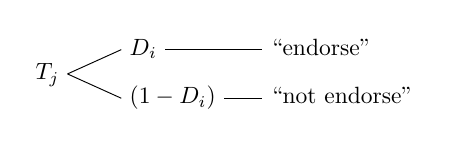
\begin{tikzpicture}[scale=0.85]
\tikzset{grow'=right}
\tikzset{execute at begin node=\strut}
\tikzset{every tree node/.style={anchor=base west}}
\tikzset{level 1/.style={level distance=40pt}}
\tikzset{level 2/.style={level distance=60pt}}
\tikzset{level 3+/.style={level distance=40pt}}
\Tree [.{$T_j$} 
   [.\node{$D_i$}; \edge; \node{``endorse''}; ]
   [.\node{$\left(1-D_i\right)$}; \edge; {``not endorse''} ]
] 
\end{tikzpicture}
      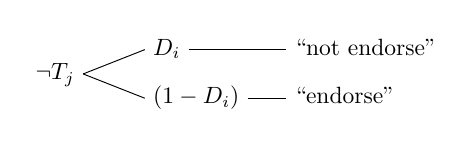
\begin{tikzpicture}[scale=0.85]
\tikzset{grow'=right}
\tikzset{execute at begin node=\strut}
\tikzset{every tree node/.style={anchor=base west}}
\tikzset{level 1/.style={level distance=50pt}}
\tikzset{level 2/.style={level distance=60pt}}
\tikzset{level 3+/.style={level distance=40pt}}
\Tree [.{$\lnot T_j$}
  [.\node{$D_i$};\edge; {``not endorse''} ]
  [.\node{$\left(1-D_i\right)$}; \edge;	{``endorse''} ]
] 
\end{tikzpicture}
    \end{center}
    
    Now, $P\left(Y_{ij}=1\right) = T_jD_i + \left(1-T_j\right)\left(1-D_i\right)$
\end{frame}


\begin{frame}
    \frametitle{Key parameters of CCT}
    \begin{itemize}
        \item \textbf{Individual Competence ($D_i$):}
        \begin{itemize}
            \item Probability distribution for individual $i$'s knowledge of the tested domain.
            \item $D_i$ lives on a probability scale (0 to 1)
            \item High probability at high values: Individual knows the consensus well.
        \end{itemize}
        \item \textbf{Item Answers/Cultural Truth ($T_j$):}
        \begin{itemize}
            \item Probability distribution for the correct answer to question $j$.
            \item Reflects the estimated consensus or collective understanding.
        \end{itemize}
    \end{itemize}
\end{frame}


\begin{frame}
    \frametitle{Model identification}
    
  Basic CCT has a tricky identification issue---that sometimes pops up when multiple unknown interact---called \emph{label switching}\pause
   
   Take $P\left(Y_{ij}=1\right) = T_jD_i + \left(1-T_j\right)\left(1-D_i\right)$\pause

   Now suppose all respondents are low in competence and all true items are false: $T_j' = 1 - T_j$ and $D'_i = 1-D_i$:\pause
\begin{eqnarray*}
  P\left(Y_{ij} = 1\right) &=& T'_jD'_i + \left(1-T'_j\right)\left(1-D'_i\right)\\\pause
  &=& (1-T_j)(1-D_i) + (1-(1-T_j))(1-(1-D_i)) \\ \pause% Substitute
  &=& (1-T_j)(1-D_i) + T_j D_i \\ \pause% Simplify
  &=& T_j D_i + (1-T_j)(1-D_i) % Rearrange
\end{eqnarray*}\pause

This makes the same predictions!
\end{frame}


\begin{frame}
    \frametitle{Handling ``Don't Know'' Responses}
    \begin{itemize}
        \item What if informants are unsure? 
        \item An explicit ``Don't Know'' (DK) option is useful.
        \item CCT models can be extended to include a process for DK responses
        \item Model accounts for the possibility that an informant:
        \begin{itemize}
            \item Gives the correct answer (if competent).
            \item If not, selects ``Don't Know'' with some probability, or...
            \item ... Guesses randomly
        \end{itemize}
        \item \textit{Benefits:}
        \begin{itemize}
            \item Provides a more accurate model of response behavior.
            \item Reduces bias caused by forced choices.
            \item Identifies true lack of knowledge or uncertainty vs.\ guessing incorrectly.
        \item Can estimate the probability of guessing vs.\ knowing/DK.
        \end{itemize}
    \end{itemize}
\end{frame}


\begin{frame}
    \frametitle{Example: Cultural Models of Illness}
    \begin{itemize}
        \item \textbf{Study:} Understanding local knowledge about diseases (e.g., diarrhea) symptoms, causes, and treatments in different communities.
        \item \textbf{Method:} Used CCT on yes/no questions about symptoms and treatments.
        \item \textbf{Findings:} Identified widely shared models of illness within cultures and variations between cultures. Estimated individual knowledge.
        \item \textbf{Use:} Essential for effective public health interventions, understanding treatment seeking behavior, and communication strategies.
    \end{itemize}
\end{frame}

\begin{frame}
    \frametitle{Example: Perceptions of Environmental Hazards}
    \begin{itemize}
        \item \textbf{Study:} Investigating shared perceptions of risks related to environmental issues (e.g., climate change, water contamination) in specific communities.
        \item \textbf{Method:} Applied CCT to understand consensus on causes, impacts, and solutions.
        \item \textbf{Findings:} Revealed differences in consensus levels across different types of risks and identified key informants.
        \item \textbf{Use:} Informs risk communication strategies, resource management plans, and community engagement efforts by tailoring messages to local knowledge.
    \end{itemize}
\end{frame}

\begin{frame}
    \frametitle{Beyond Single Consensus: Multiple Subcultures}
    \begin{itemize}
        \item The basic CCT assumes a single dominant ``truth.''
        \item What if the agreement patterns suggest multiple distinct viewpoints or subcultures?
        \item \textbf{Multiple Consensus Models:} Extensions that look for evidence of multiple latent factors in the agreement data.
        \item Bayesian frameworks are flexible and can be adapted to estimate parameters for multiple potential consensus models simultaneously.
    \end{itemize}
\end{frame}


\begin{frame}
    \frametitle{Summary}
    \begin{itemize}
        \item Cultural Consensus Theory offers a powerful way to measure what is collectively known or believed in a group.
        \item The Bayesian approach provides a robust method that explicitly models uncertainty and can handle complexities like ``Don't Know'' responses.
        \item By analyzing agreement patterns, we can identify shared knowledge and the individuals who are most knowledgeable within that domain.
        \item It's a valuable but slightly underappreciated tool for researchers across social sciences and applied fields seeking to understand shared cognition.
    \end{itemize}
\end{frame}


\maketitle

\end{document}